\section{Binomial distribution ($X \sim  B(n,p)$)}

\begin{table}[H]
    \hfill
    \begin{minipage}{0.45\linewidth}
        \begin{figure}[H]
            \centering
            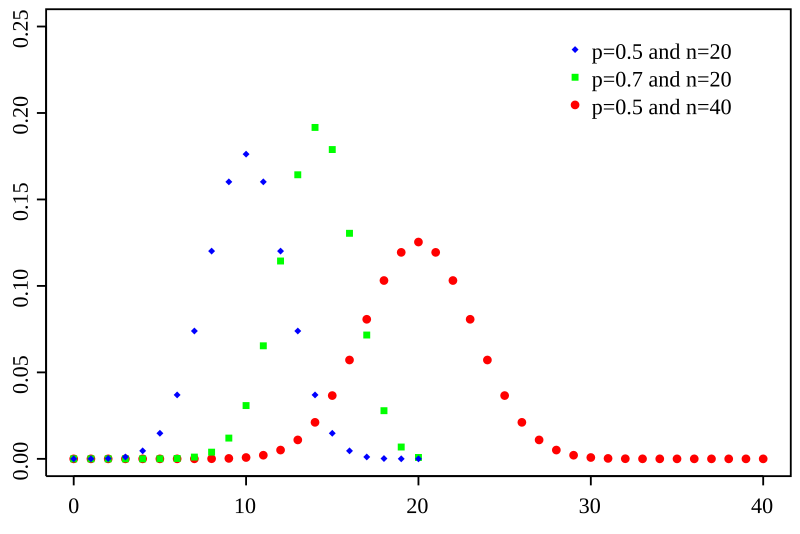
\includegraphics[
                width=\linewidth,
                height=5cm,
                keepaspectratio,
            ]{images/distributions/Binomial_distribution_pmf.svg.png}
            \caption{Binomial Distribution: PDF \cite{wiki/Binomial_distribution}}
        \end{figure}
    \end{minipage}
    \hfill
    \begin{minipage}{0.45\linewidth}
        \begin{figure}[H]
            \centering
            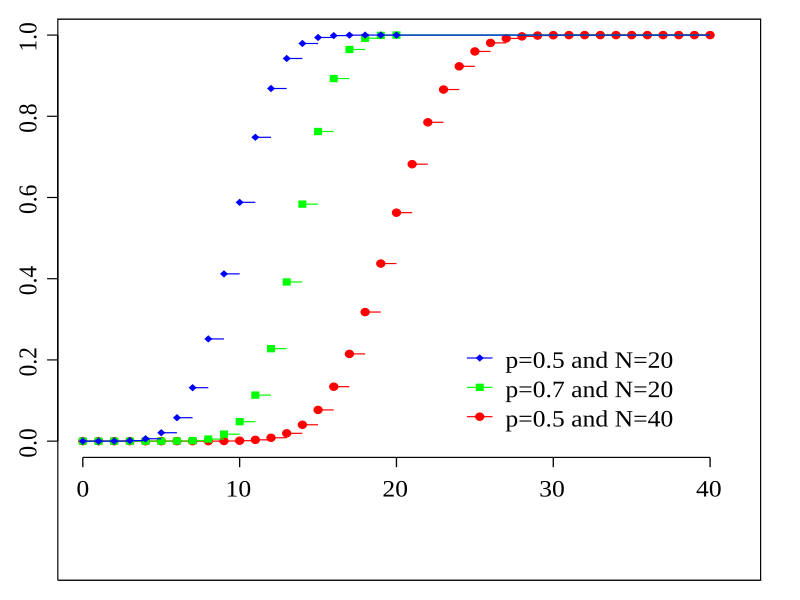
\includegraphics[
                width=\linewidth,
                height=5cm,
                keepaspectratio,
            ]{images/distributions/Binomial_distribution_cdf.svg.png}
            \caption{Binomial Distribution: CDF \cite{wiki/Binomial_distribution}}
        \end{figure}
    \end{minipage}
    \hfill
\end{table}





\begin{enumerate}
    \item A \textbf{disadvantage} of a random variable with a binomial distribution function is that it is bounded by the number of trials $n$.
    \hfill \cite{statistics/book/Statistics-for-Data-Scientists/Maurits-Kaptein}
\end{enumerate}





\subsection{PMF}

\begin{enumerate}
    \item binomial random variable $S_n$ is the sum of $n$ independent Bernoulli variables
    \hfill \cite{statistics/book/Statistics-for-Data-Scientists/Maurits-Kaptein}

    \item The random variable $S_n$ is then given by $S_n = X_1 + X_2 + \cdots + X _n$ , with $X_ k$ the binary random variable for turn $k$
    \hfill \cite{statistics/book/Statistics-for-Data-Scientists/Maurits-Kaptein}

    \item The PMF of the binomial is given by:
    \hfill \cite{statistics/book/Statistics-for-Data-Scientists/Maurits-Kaptein}
    \\
    $
        P(S_n = s)
        = f_{n,p}(s)
        = \displaystyle\binom{n}{s} p^s (1-p)^{n-s}
    $
    \hfill
    $
        \displaystyle\binom{n}{s} = \dfrac{n!}{s!(n-s)!}
    $
    \hfill \cite{statistics/book/Statistics-for-Data-Scientists/Maurits-Kaptein}
\end{enumerate}






\subsection{Summary}

\begin{enumerate}
    \item \textbf{Notation}:
    $
         {\displaystyle \mathcal{B}(n,p)}
    $
    \hfill \cite{wiki/Binomial_distribution}

    \item \textbf{Parameters}:
    \begin{enumerate}
        \item ${\displaystyle n\in \{0,1,2,\ldots \}}$ – number of trials
        \hfill \cite{wiki/Binomial_distribution}

        \item ${\displaystyle p\in [0,1]}$ – success probability for each trial
        \hfill \cite{wiki/Binomial_distribution}

        \item ${\displaystyle q=1-p}$ - failure probability for each trial
        \hfill \cite{wiki/Binomial_distribution}
    \end{enumerate}
    \hfill \cite{wiki/Binomial_distribution}

    \item \textbf{Support}:
     ${\displaystyle k\in \{0,1,\ldots ,n\}}$ – number of successes
    \hfill \cite{wiki/Binomial_distribution}

    \item \textbf{PMF}:
    $
         {\displaystyle {\binom {n}{k}}p^{k}q^{n-k}}
    $
    \hfill \cite{wiki/Binomial_distribution}

    \item \textbf{CDF}:
     ${\displaystyle I_{q}(n-\lfloor k\rfloor ,1+\lfloor k\rfloor )}$ (the regularized incomplete beta function)
    \hfill \cite{wiki/Binomial_distribution}

    \item \textbf{Mean}:
    $
         {\displaystyle np}
    $
    \hfill \cite{wiki/Binomial_distribution}

    \item \textbf{Median}:
    ${\displaystyle \lfloor np\rfloor }$ or ${\displaystyle \lceil np\rceil }$
    \hfill \cite{wiki/Binomial_distribution}

    \item \textbf{Mode}:
     ${\displaystyle \lfloor (n+1)p\rfloor }$ or ${\displaystyle \lceil (n+1)p\rceil -1}$
    \hfill \cite{wiki/Binomial_distribution}

    \item \textbf{Variance}:
    $
         {\displaystyle npq=np(1-p)}
    $
    \hfill \cite{wiki/Binomial_distribution}

    % \item \textbf{Median absolute deviation (MAD)}:
    % $

    % $
    % \hfill \cite{wiki/Binomial_distribution}

    \item \textbf{Skewness}:
    $
         {\displaystyle {\dfrac {q-p}{\sqrt {npq}}}}
    $
    \hfill \cite{wiki/Binomial_distribution}

    \item \textbf{Excess kurtosis}:
    $
         {\displaystyle {\dfrac {1-6pq}{npq}}}
    $
    \hfill \cite{wiki/Binomial_distribution}

    \item \textbf{Entropy}:
     ${\displaystyle {\dfrac {1}{2}}\log _{2}(2\pi enpq)+O\left({\dfrac {1}{n}}\right)}$ in shannons. For nats, use the natural log in the log.
    \hfill \cite{wiki/Binomial_distribution}

    \item \textbf{Moment-generating function (MGF)}:
    $
         {\displaystyle (q+pe^{t})^{n}}
    $
    \hfill \cite{wiki/Binomial_distribution}

    \item \textbf{Characteristic function (CF)}:
    $
         {\displaystyle (q+pe^{it})^{n}}
    $
    \hfill \cite{wiki/Binomial_distribution}

    \item \textbf{Probability-generating function (PGF)}:
    $
         {\displaystyle G(z)=[q+pz]^{n}}
    $
    \hfill \cite{wiki/Binomial_distribution}

    \item \textbf{Fisher information}:
    ${\displaystyle g_{n}(p)={\dfrac {n}{pq}}}$ (for fixed n ${\displaystyle n}$)
    \hfill \cite{wiki/Binomial_distribution}
\end{enumerate}





